\documentclass[16.7pt]{jsarticle}

\usepackage{SPR}
\usepackage{comment}
\headerSPR
\begin{document}
	\titleSPR{\number\year}{\number\month}{\number\day}{D2}{吉田 皓太郎}
%%%%%%%%%%%%%%%%%%%%%%%%%%%%%%%%%%%%%%
	%\articleSPRabst
	%	\begin{itemize}
	%		\item =どういう事態か
	%	\end{itemize}
		
%今回のMTGの目的,何をディスカッションし,結果に何を得たいのかを決定する.※ミーティングごとに記入
	\articleSPRobj
		今回のMTGでは,誤差要因に関する考察を三度考察し,まとめるものである.これを通したディスカッションにより,結果の妥当性などを確認していきたいと考えている.
		

%%%%%%%%%%%%%%%%%%%%%%%%%%%%%%%%%%%%%%
% 1.前回からのノルマ
	\articleSPRitemsone
		%\begin{enumerate}
		%	\item A
		%\end{enumerate}
		
		\tableofcontents
		
		
%%%%%%%%%%%%%%%%%%%%%%%%%%%%%%%%%%%%%%
%\begin{itemize}
%	\item 新規手法について
%	\item ISFAアウトライン
%\end{itemize}
%%%%%%%%%%%%%%%%%%%%%%%%%%%%%%%%%%%%%%
% 2.具体的な成果
	\articleSPRitemstwo
	\renewcommand{\labelitemi}{$\blacktriangledown$}
	%\renewcommand{\labelitemi}{$\bigcirc$}
	\newcommand{\argmax}{\mathop{\rm arg~max}\limits}
	\newcommand{\argmin}{\mathop{\rm arg~min}\limits}
	\newcommand{\Ker}{{\rm Ker}}
	\newcommand{\rank}{{\rm rank}}
%%%%%%%%%%%%%%%%%%%%%%%%%%%%%%%%%%%%%
\section{データ周りの話について}
		\subsection{前回の研究会までで行ったこと}
		前回の考察では,主にデータ間の距離に着目し,議論を進めた.しかし,ガウス過程回帰により得られたパラメータにおける話の整合性が薄かった点や,内挿および外挿的な部分が議論できていないなど,詰めるべき課題が多く残っていた.
		
		まずはじめに考察したのは,内挿と外挿の話であった.内挿と外挿を定義するため,入力データの凸包を考え,凸包内に出力データが入っていなければ外挿というアイデアを考えたが,計算結果として,少なくとも凸包内には全ての出力データは含まれるという結果しか得られなかったため,頓挫.
		
		ここで,改めてテストデータに対する予測値の絶対誤差と分散をまとめたものを示す.
		
		\begin{figure}[h]
			\centering
				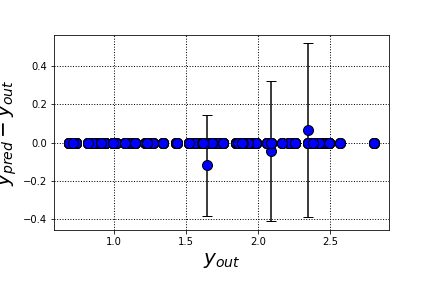
\includegraphics[width= 0.5\columnwidth]{./figure/ERR_WITH_VARS2.png}
			\caption{Manhattan}
		\end{figure}
	
		この結果から,例え入力パラメータが異なっていても,出力値は似たような値を取ることが多い.という事象が読み取れる.このことから,1つの仮説を導く.
		\subsection{仮説}
		このデータの意味する所を,整理すれば,
		\begin{itemize}
			\item 誤差が大きい評価値においても,似たような評価値を出力する別の入力パラメータが存在する.
		\end{itemize}
		となる.ここから,今回扱う問題の性質として以下を得る.
		\begin{itemize}
			\item 入力形状に対する評価値は,単射ではない.
		\end{itemize}
		単射を概説する.ある集合$ \bd{X},\bd{Y} $に対して対応$ f:\bd{X}\rightarrow \bd{Y} $が与えられている場合,$ \bd{X} $の任意の2元$ \bd{x},\bd{x}' $をどのようにとっても,$ f(\bd{x}) \neq f(\bd{x}') $が成り立つことを単射であるという.
		
		今回の評価値の成り立ちについて考えれば,カップの囲う体積と面積を割ることで決まる評価値であり,関数の単射性が成立しないのは,自然で不都合はないと思われる.
		\begin{figure}[h]
			\centering
			\begin{minipage}{0.45\hsize}
				\centering
				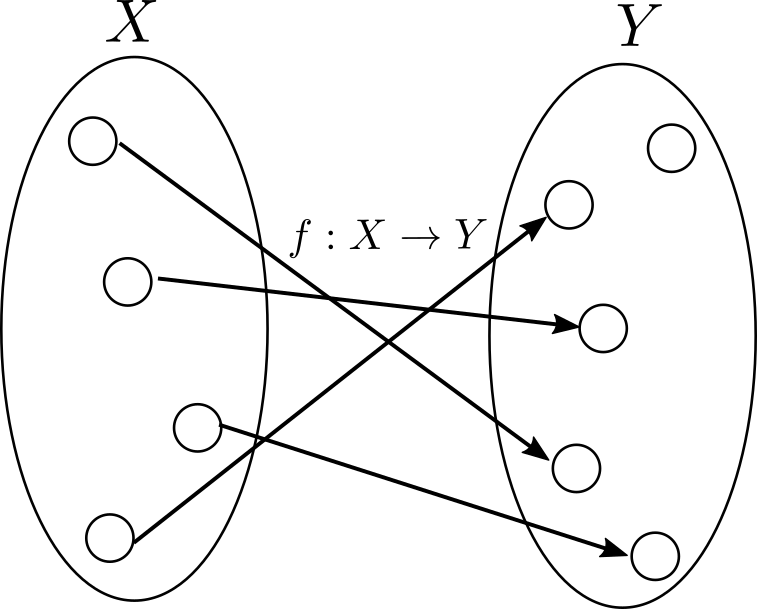
\includegraphics[width= 0.65\columnwidth]{./figure/Injection.png}
				\caption{単射}
			\end{minipage}
			\begin{minipage}{0.45\hsize}
				\centering
				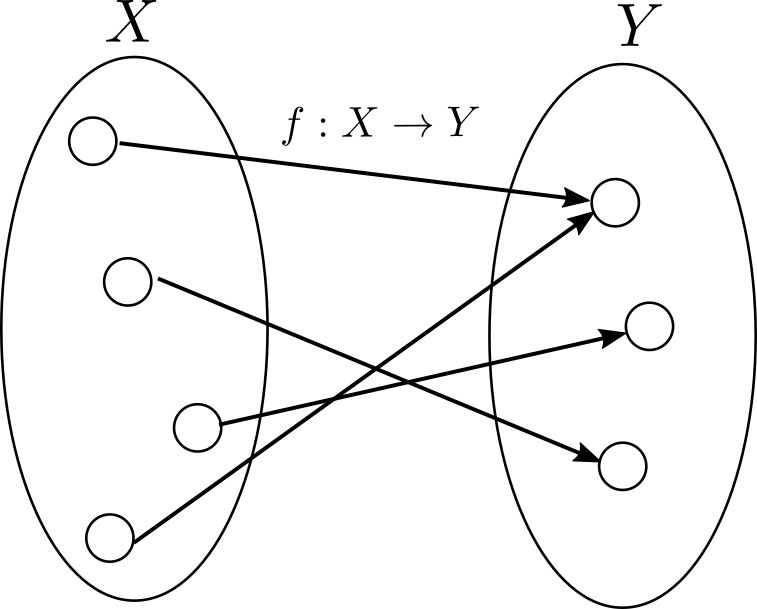
\includegraphics[width= 0.65\columnwidth]{./figure/Surjection.png}
				\caption{単射ではない}
			\end{minipage}
		\end{figure}
		
		ここから導いた仮説は
		\begin{itemize}
			\item 検証データにおける誤差の大きな値をとった出力値における入力値は,訓練データにおいて似たような出力値における入力値と似ていなかったため,誤差が発生した.
		\end{itemize}
		例えば,$ y=\sin x $において,$ x \in [0,2\pi) $の区間で学習させた曲線を考える.この時データのばらつきによっては,$ x = 2\pi $における出力は,必ずしも期待値である$ 0 $と予測できないと考えられる.この時,訓練データの入力パラメータ群に対して,データとの距離だけで見れば小さいが,ある意味外挿的であると考えられる.そこで,この考え方を用いて考察してみる.
		\subsection{数値実験内容}
		今回はこの仮説を基にして,以下のように実験を行った.以下では,訓練データ集合を$ \bd{D} = (\bd{X},\bd{y}) $と表現し,検証データ集合を$ \bd{D}^* = (\bd{X}^*,\bd{y}^*) $として表現する.
		\begin{enumerate}
			\item 検証データにおける入力パラメータ集合$ \bd{X}^* $の全ての元$ \bd{x}^*$に対して,近傍データセット$ \bd{U}(\bd{D}) $を決定する.
			\item $ \bd{U}(\bd{D}) $に対する最短距離$ \delta $を求める.この$ \delta $が大きければ大きいほど,乖離が激しく,$ \bd{x}^* $は外挿的なデータであると判断できる.
		\end{enumerate}
		近傍$ \bd{U}(\bd{D}) $は,以下のように定義される集合である.
		\begin{equation}\label{eq:Neighborhood}
			\bd{U}(\bd{D}) = \{ (\bd{x},y) \in \bd{D}| |y-y^*| \leq \varepsilon \}
		\end{equation}
	
		\begin{figure}[h]
			\centering
			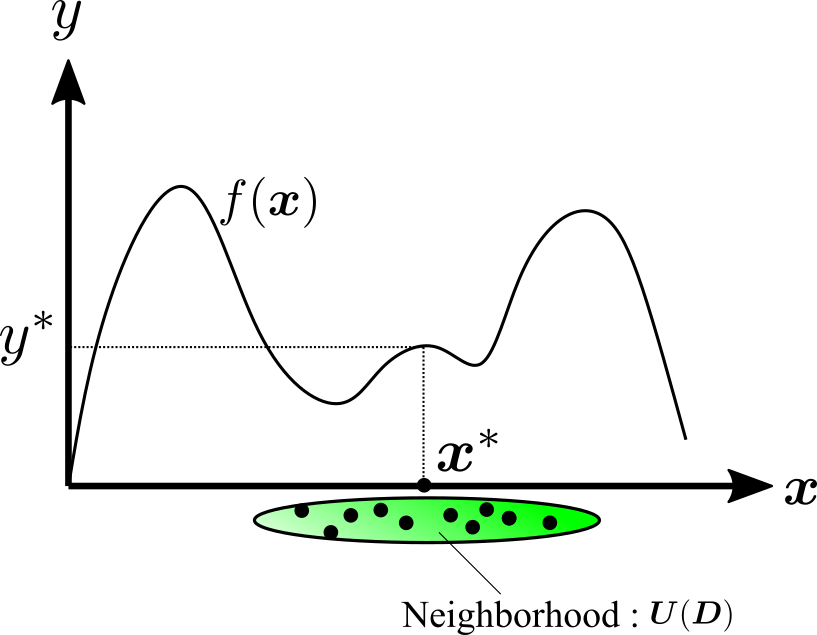
\includegraphics[width= 0.55\columnwidth]{./figure/Neighborhood.png}
			\caption{Manhattan}
		\end{figure}
		また,$ \delta $は以下のように定義する.
		\begin{equation}\label{eq:delta_eq}
			\delta = \min_{\bd{u} \in \bd{U}(\bd{D})} d(\bd{u},\bd{x}^*)
		\end{equation}
		今回は,$ \varepsilon = 0.02 $とし,距離空間には,先月の結果から,マンハッタン距離を採用する.
		
		これを用いて全体のパラメータを用いて計算した結果と,各$ \alpha,\omega_{\eta},D $のそれぞれで分けて計算した結果を,以下に示す.
		
		\begin{figure}[h]
			\centering
			\begin{minipage}{0.45\hsize}
				\centering
				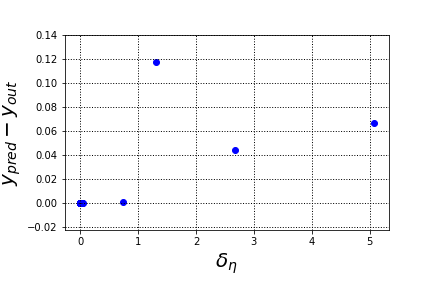
\includegraphics[width= 0.85\columnwidth]{./figure/delta_OmgEta.png}
				\caption{$ \omega_{\eta} $}
			\end{minipage}
			\begin{minipage}{0.45\hsize}
				\centering
				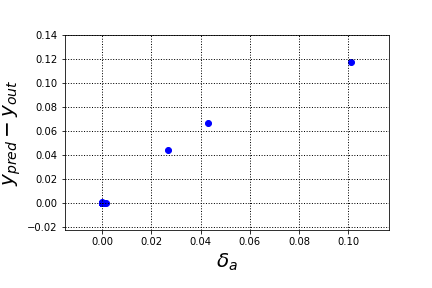
\includegraphics[width= 0.85\columnwidth]{./figure/delta_Alpha.png}
				\caption{$ \alpha $}
			\end{minipage}
			\begin{minipage}{0.45\hsize}
				\centering
				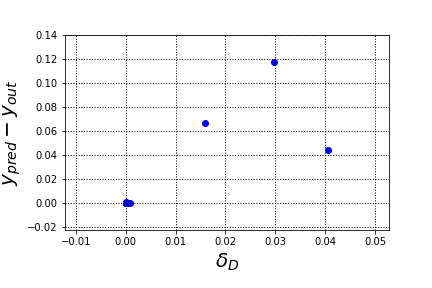
\includegraphics[width= 0.85\columnwidth]{./figure/delta_Dist.png}
				\caption{$ D $}
			\end{minipage}
			\begin{minipage}{0.45\hsize}
				\centering
				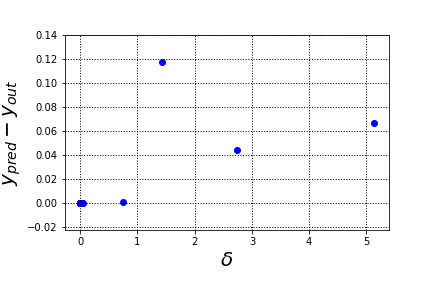
\includegraphics[width= 0.85\columnwidth]{./figure/ERR_DELTA.png}
				\caption{All Params}
			\end{minipage}
		\caption{Regarding Abs Err}
		\end{figure}
		
		\begin{figure}[h]
			\centering
			\begin{minipage}{0.45\hsize}
				\centering
				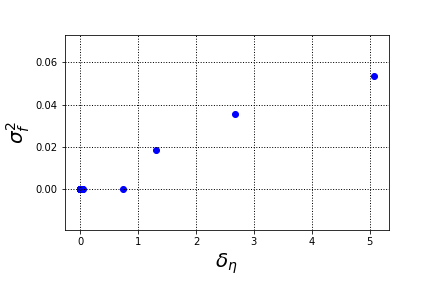
\includegraphics[width= 0.85\columnwidth]{./figure/vars_OmgEta.png}
				\caption{$ \omega_{\eta} $}
			\end{minipage}
			\begin{minipage}{0.45\hsize}
				\centering
				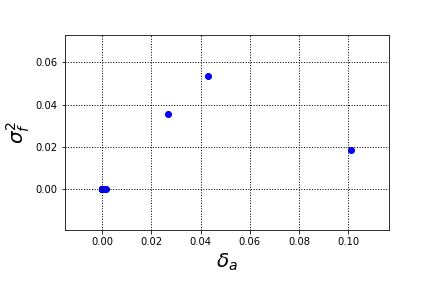
\includegraphics[width= 0.85\columnwidth]{./figure/vars_Alpha.png}
				\caption{$ \alpha $}
			\end{minipage}
			\begin{minipage}{0.45\hsize}
				\centering
				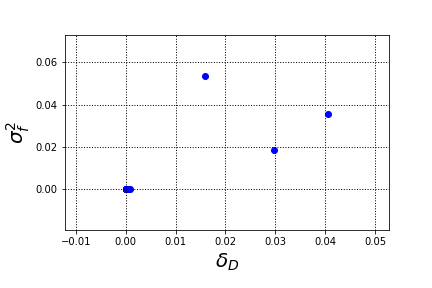
\includegraphics[width= 0.85\columnwidth]{./figure/vars_Dist.png}
				\caption{$ D $}
			\end{minipage}
			\begin{minipage}{0.45\hsize}
				\centering
				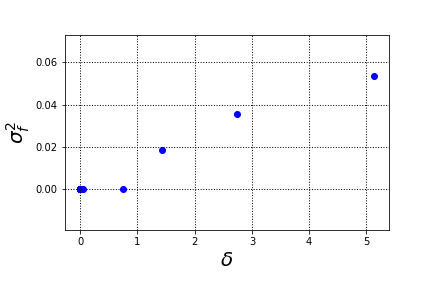
\includegraphics[width= 0.85\columnwidth]{./figure/ERR_VARS.png}
				\caption{All Params}
			\end{minipage}
			\caption{Regarding Vars}
		\end{figure}
	前回の結果では,データの距離が大きい部分があっても,誤差や分散が小さい例があったが,今回の場合にはそのようなことがなく,ほぼ正確に距離との相関が確認される.
	
	個別の例では,絶対誤差と特に$ \alpha $の比例関係が確認される.これは,以前示したガウス過程回帰によって得られたパラメータ群における考察の結果である,$ \alpha $が重要なパラメータであるという事実に矛盾しない結果となった.
	
	全体のパラメータで見ると,データの曖昧さを表現している分散の大きさと距離がほぼ完全な比例関係にあることが読み取れる.つまり,外挿的であればあるほど,得られる解の信頼度に揺らぎが生じるという結果を得た.
	
	上記の内容は,研究会や査読に対して突っ込まれた際にも応用できるかと思いますが,いかがでしょうか.(言葉を整理する必要はありますが・・・)
\begin{comment}
	\subsection{前提}
今回のパラメータは,関数$ \alpha,\omega_{\eta},D $がそれぞれ,(仮定的に)ノイズを含んだ独立ガウス過程$ N(\bd{0},\bd{K} + \sigma^2 \bd{I}) $に従って出力されているとする.$ \bd{K} $はグラム行列を表しており,各成分を定義するカーネル関数$ k(\bd{x}_i,\bd{x}_j) $を設計することにより得る.
\subsection{考察}
まず初めに,特徴パラメータからガウス過程を用いて回帰させた際のハイパーパラメータに関する考察から行う.
今回ガウス過程を適用する際に使用したカーネル関数は以下のように,RBF関数と線形関数を組み合わせたARD(関連度自動決定)カーネル関数である.ARD関数は,パラメータ毎に重みが変化し,評価値に対する相関度を自動的に決定することができる.
\begin{equation}\label{eq:ARD_Kernel}
k(\bd{x}_i,\bd{x}_j) = \theta_1 \exp \left[(\bd{x}_i - \bd{x}_j)^T  diag(\bd{\Theta}_R)^{-1}  (\bd{x}_i - \bd{x}_j) \right] + \bd{x}_i^T diag(\bd{\Theta}_L) \bd{x}_j
\end{equation}
ここで$ diag(\bd{\Theta}) $は,ベクトル$ \Theta $の各成分を対角成分に持つ対角行列である.ARDの場合は,$ \dim \bd{\Theta}_L = \dim \bd{\Theta}_R =  \dim \bd{x} $となる.

また,今回特徴パラメータを抽出する際に用いたガウス過程のカーネル関数はRBF関数であったことから,1つの関数につき三つのパラメータ$ \theta_1,\theta_2,\sigma $を得る.
今回得られた$ \Theta_L,\Theta_R $を表にまとめると,次の通りとなった.

\begin{table}[h]
\centering
\begin{tabular}{|c|c|c|c|}
\hline
& $\alpha$ & $\omega_{\eta}$ & D        \\ \hline
$\bd{\Theta}_{R,0}$        & 0.065274                      & 0.047916                             & 0.266596               \\ \hline
$\bd{\Theta}_{R,1}$ & 158.2779                      & 5.668934                             & 0.286779               \\ \hline
$\bd{\Theta}_{R,2}$ & 1                             & 318.7759                             & 1                    \\ \hline
\end{tabular}
\end{table}

\begin{table}[h]
\centering
\begin{tabular}{|c|c|c|c|}
\hline
& $\alpha$ & $\omega_{\eta}$ & $D$       \\ \hline
$\bd{\Theta}_{L,0}$        & $9.827\times 10^{-3}$ & $1.219\times 10^{-4}$        & $1.083\times 10^{-6}$ \\ \hline
$\bd{\Theta}_{L,1}$ & $2.920\times 10^{1}$ & $8.416\times 10^{-3}$        & $1.420\times 10^{1}$ \\ \hline
$\bd{\Theta}_{L,2}$ & $1.000$    & $2.732$        & $1.000$   \\ \hline
\end{tabular}
\end{table}
この結果から,特に$ \omega_{\eta} $の分散に対して関連度が高いことが読み取れる.
\end{comment}
	
		
%		まず初めに,特徴パラメータからガウス過程を用いて回帰させた際のハイパーパラメータに関する考察から行う.
%		今回ガウス過程を適用する際に使用したカーネル関数は以下のように,RBF関数と線形関数を組み合わせたARD(関連度自動決定)カーネル関数である.ARD関数は,パラメータ毎に重みが変化し,評価値に対する相関度を自動的に決定することができる.
%		\begin{equation}\label{eq:ARD_Kernel}
%			k(\bd{x}_i,\bd{x}_j) = \theta_1 \exp \left[(\bd{x}_i - \bd{x}_j)^T  diag(\bd{\Theta}_R)^{-1}  (\bd{x}_i - %\bd{x}_j) \right] + \bd{x}_i^T diag(\bd{\Theta}_L) \bd{x}_j
%		\end{equation}
%		ここで$ diag(\bd{\Theta}) $は,ベクトル$ \Theta $の各成分を対角成分に持つ対角行列である.ARDの場合は,$ \dim \bd{\Theta}_L = \dim \bd{\Theta}_R =  \dim \bd{x} $となる.
		
%		また,今回特徴パラメータを抽出する際に用いたガウス過程のカーネル関数はRBF関数であったことから,1つの関数につき三つのパラメータ$ \theta_1,\theta_2,\sigma $を得る.
%		今回得られた$ \Theta_L,\Theta_R $を表にまとめると,次の通りとなった.
		
%		\begin{table}[h]
%			\centering
%			\begin{tabular}{|c|c|c|c|}
%				\hline
%				& $\alpha$ & $\omega_{\eta}$ & D        \\ \hline
%				$\bd{\Theta}_{R,0}$        & $1.532\times 10^1$ & $2.087\times 10^1$        & $3.751\times %10^1$ \\ \hline
%				$\bd{\Theta}_{R,1}$ & $6.318\times 10^{-3}$ & $1.764\times 10^{-1}$        & $3.487\times 10^{-2}$ \\ \hline
%				$\bd{\Theta}_{R,2}$ & $1.000$    & $3.137\times 10^{-3}$        & $1.000$   \\ \hline
%			\end{tabular}
%		\end{table}
	
%		\begin{table}[h]
%			\centering
%			\begin{tabular}{|c|c|c|c|}
%				\hline
%				& $\alpha$ & $\omega_{\eta}$ & $D$       \\ \hline
%				$\bd{\Theta}_{L,0}$        & $9.827\times 10^{-3}$ & $1.219\times 10^{-4}$        & $1.083\times 10^{-6}$ \\ \hline
%				$\bd{\Theta}_{L,1}$ & $2.920\times 10^{1}$ & $8.416\times 10^{-3}$        & $1.420\times 10^{1}$ \\ \hline
%				$\bd{\Theta}_{L,2}$ & $1.000$    & $2.732$        & $1.000$   \\ \hline
%			\end{tabular}
%		\end{table}
%	$\bd{\Theta}_{R,i} (i=0,1,2)$に対するパラメータの計算オーダーは以下のようになる.
%	\begin{table}[h]
%		\centering
%		\begin{tabular}{|c|c|c|c|}
%			\hline
%			& $\alpha$ & $\omega_{\eta}$ & $D$        \\ \hline
%			$\bd{\Theta}_{L,0}$        &   $10^{-2}$& $10^{0}$        & $10^{-2}$ \\ \hline
%			$\bd{\Theta}_{L,1}$ & $ 10^{-1}$ & $10^{-1}$        & $10^{-1}$ \\ \hline
%			$\bd{\Theta}_{L,2}$ & $10^{-15}$    & $10^{-3}$        & $10^{-16}$   \\ \hline
%		\end{tabular}
%	\end{table}
%	となっている.
	
%	この事を考慮すると,$ \alpha $に対する特徴パラメータの差分に対してカーネル関数の値が他の値に対して大きく変化することが分かる.すなわち今回の評価関数は,主に$ \alpha $が支配的な要因であることが読み取れる.
	
%	仮にデータの疎密性がデータ間の距離に対して強く相関関係にあるとすれば,疎密性を定義することは,データ間の距離をうまく定義することに等しくなるため,これについて考える.
	
%	今回はデータの距離を定義するにあたって,2つの距離を用いて,$ \alpha $の特徴パラメータに対する評価誤差について考察を行った.
	
%	今回用いるパラメータは,オーダーのばらつきが大きいことから,1つ目はチェベシェフ距離を採用する.
	\section{次回のMTGについて(終了後記載)}
	\begin{itemize}
		\item  
		\item 
	\end{itemize}
	###
	\newpage
%\vspace{10cm}
%%%%%%%%%%%%%%%%%%%%%%%%%%%%%%%%%%%%%%
% 3.達成できなかったこととその問題点
	%\articleSPRthree
	
%%%%%%%%%%%%%%%%%%%%%%%%%%%%%%%%%%%%%%

%\vspace{14cm}
%%%%%%%%%%%%%%%%%%%%%%%%%%%%%%%%%%%%%%
	%\articleSPRfour
	%\articleSPRfive
\end{document}
